\documentclass[journal]{IEEEtran}
\IEEEoverridecommandlockouts
\usepackage{cite}
\usepackage{amsmath,amssymb,amsfonts}
\usepackage{algorithmic}
\usepackage{graphicx}
\graphicspath{{./design/pdf-snapshots/cropped/}{./assets/}{./design/video-output/noise-identification/}{./design/video-output/noisy-image/}{./design/video-output/post-nr/}{./design/video-output/reference/}}
\usepackage{textcomp}
\usepackage{xcolor}
\usepackage{float}
\usepackage{grffile}
\usepackage{hyperref}
\usepackage{lipsum}
\ifCLASSOPTIONcompsoc
\usepackage[caption=false, font=normalsize, labelfont=sf, textfont=sf]{subfig}
\else
\usepackage[caption=false, font=footnotesize]{subfig}
\fi
\def\BibTeX{{\rm B\kern-.05em{\sc i\kern-.025em b}\kern-.08em
    T\kern-.1667em\lower.7ex\hbox{E}\kern-.125emX}}
    
\newcommand{\textregisteredmark}{\textsuperscript{\tiny\textregistered}}
\renewcommand{\figureautorefname}{Fig.}
\newcommand{\subfigureautorefname}{\figureautorefname}

\begin{document}

\title{Correction Techniques for Image Faults}

\author{Dominic~Gaiero,~\textit{\href{mailto:dgaiero@calpoly.edu}{dgaiero@calpoly.edu}}
    Nicholas Serres,~\textit{\href{mailto:nserres@calopoly.edu}{nserres@calpoly.edu}}}

\maketitle

\begin{abstract}
Faults in image sensors can lead to a large drop in image reliability and quality. Image sensors are one of the most susceptible components to faults, and is one critical components in a camera system. This paper explores fault detection and correction of an image sensor by analyzing a sequence of frames from the camera to identify permanent faults and correct both permanent and transient faults. This paper is focused on applications in extreme environments, but applies to wider fields. 
\end{abstract}

\section{Introduction}
\IEEEPARstart{I}{n} this paper the effectiveness of detecting and correcting radiation-induced errors in an image sensor is explored. This provides an alternative on past methods by correcting and detecting faults in the image processing module, rather than a hardware level redesign. While using software to mitigate the effects of radiation on sensors is not a permanent solution, the benefits of significant reduced costs and development make this solution  appealing for non-critical applications. This project targets uses in control cameras at a radiation plants or other radiation intensive conditions where fault mitigation is desired. This will allow systems that use cameras in these conditions to operate with higher reliability and provide higher fidelity imagery despite the operating conditions of the cameras. Additionally, this solution provides enhanced reporting to the end user, unlike traditional image processing techniques.
\section{CMOS Background}
%% Can you also try and add some paragraphs? You can use the \par command.

CMOS(complementary metal oxide semiconductor) sensors are one of the most commonly used modern methods of creating digital images in cameras.  \autoref{fig:filters} illustrates how light passing from the outside passes through a glass lens and a color filter before finally reaching the photo-diodes.
\begin{figure}[H]
    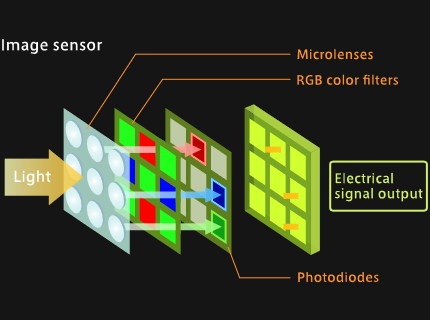
\includegraphics[scale= .5]{assets/ImageSensor.png}
    \caption{CMOS Image Sensor}
    \label{fig:filters}
\end{figure}
The photo-diode is sensitive to light and is able to generate a current by being exposed to photons.  Finally that signal is sent to a central processor and translated into a pixel.(Tokyo Electron Museum)  CMOS sensors are very vulnerable to faults due to radiation and other interference because in some way the circuit has to be exposed to incoming rays and cannot be fully insulated. \autoref{fig:CMOS} shows a basic schematic for a CMOS sensor.  The photo diode has to be exposed to the incoming light so that it can activate the circuit, however, this makes it vulnerable to any other interference that can potentially harm the sensor.  
\begin{figure}[H]
    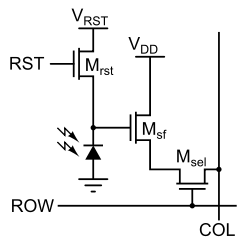
\includegraphics[scale= .75]{assets/Cmos schemateic.png}
    \caption{Basic CMOS Active Pixel}
    \label{fig:CMOS}
\end{figure}
One fault that often occurs in CMOS sensors is a Dark Current.  A dark current is when the CMOS circuit is activated by a wave that is not a photon.  In space and other radiation intensive environments this is a very relevant limitation of the technology because extreme accuracy is required with very high consistency.  Radiation that reaches a sensor is likely to cause the sensor to have some kind of fault, and if the intensity of the radiation is high enough then a pixel can become permanently damaged.  These Dark Currents when realized through the circuit and the central processor would appear to be a noisy picture or a collection of white pixels.  These faults can be harmless at first, but given enough time to build up they can render a sensor useless.
\section{Dark Currents}
Dark current is a very large limiting factor in the performance of an image sensor.  Image sensors work by generating a signal when an area of the signal has a different light level than the rest and it is able to then generate a pixel.  Dark currents "occur in every pixel, but vary from pixel-to-pixel" based on a number of factors such as heat on the image sensor.  Due to how pervasive dark currents are for image sensors there is a lot of research going into how to possibly prevent any dark currents.  Over the past 40 years there has  been nearly a 5000x drop in the dark current for image sensors, but this is still too high for many applications of image sensors.(Dan McGrath 2018)  Star trackers on sat elites need incredibly precise images to be taken on star trackers so that they can accurately calculate their position.  Any noise or dark currents induced in these sensors can results in large miscalculations.  Because some stars are so small relative to the star tracker, any noise and image can result in a failure of the star tracker.  In cases like star trackers on satellites dark current is a very dangerous fault.  
\section{Related Work} 
\input{relaedWorks}
\section{Method}
\subsection{Tools Used}
The model was designed using MATLAB\textregisteredmark\ and SIMULINK\textregisteredmark\ R2018B. Analysis was also performed using this software. Additionally, to aid testing, a generic video file was used provided by \hyperlink{https://blogs.unity3d.com/2016/11/28/free-vfx-image-sequences-flipbooks/}{Unity3D}.
\subsection{Assumptions}
The video file used has dimensions of 400x400px. Inside the parameters of certain blocks in the SIMULINK\textregisteredmark\ file this assumption was used and the model will need to be altered to work with video files of other dimensions. Additionally, the input video file was 30fps which is assumed in the frame counter module.
\subsection{Design}
The top level design is shown in \autoref{fig:sysSpecs}. Should the reader wish to download a copy of this design, the latest working copy can be found at \hyperlink{https://github.com/dgaiero/cpe-446-final-paper/blob/master/design/impl_dsgn.slx}{https://github.com/dgaiero/cpe-446-final-paper/blob/master/design/impl\_dsgn.slx}. The SIMULINK\textregisteredmark\ library used during development can also be found \hyperlink{https://github.com/dgaiero/cpe-446-final-paper/blob/master/design/library.slx}{here} A general overview of this design is presented in this section with in-depth descriptions in later sections.
\begin{figure*}
    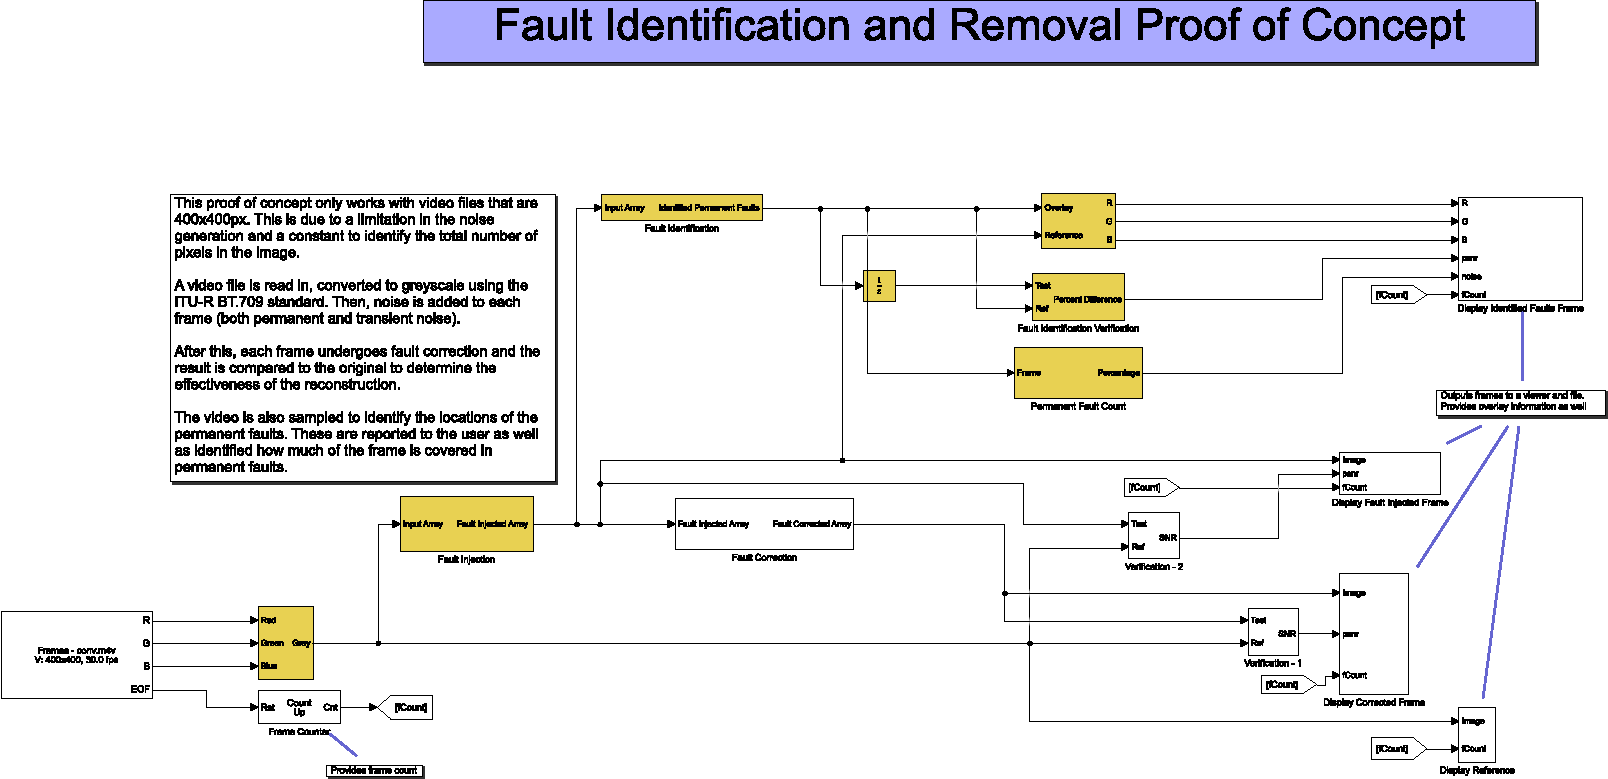
\includegraphics[width=\textwidth]{impl_dsgn}
    \caption{Top Level System Design}
    \label{fig:sysSpecs}
\end{figure*}
\par An input video is fed into the \verb!From Multimedia File! block. Each color frame is converted to black and white to make image processing easier. Additionally, the \verb!EOF! output of the \verb!From Multimedia File! is fed into a frame counter's reset port, which is reset every time the video is restarted.
\par From this point, the video is sent to a fault injection unit. Since this model is a proof of concept, it is important to have a reference video as well as a video file with faults injected. The fault injection block adds both permanent and transient faults.
\par After the frame has faults added, it is sent to two blocks, one to identify permanent faults in the frame, and another to filter out the faults in the frame.
\par Post fault injection, fault filtering, fault identification, and the reference frames are output to a video display as well as logged to a video file throughout simulation. Frame count information as well as other diagnostic and verification information is overlaid on top of the video frames to aid in analysis.
\subsubsection{ITU-R BT.709 Sub module}
The black and white conversion module follows the ITU-R BT.709 standard for color to black and white conversion. A reproduction of this module along with the coefficients used for each channel is shown in \autoref{fig:btu709}.
\begin{figure}[H]
    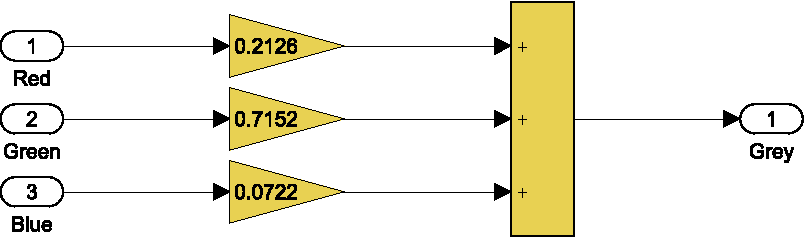
\includegraphics[width=\linewidth]{impl_dsgn_ITU-R BT.709}
    \caption{ITU-R BT.709 Color to Black and White Conversion}
    \label{fig:btu709}
\end{figure}

\subsubsection{Fault Injection Sub module}
The fault injection sub module generates both permanent and transient faults.
\begin{figure}[H]
    \subfloat[Top Level Fault Injection Block\label{fig:topLevelFaultInjector}]{%
       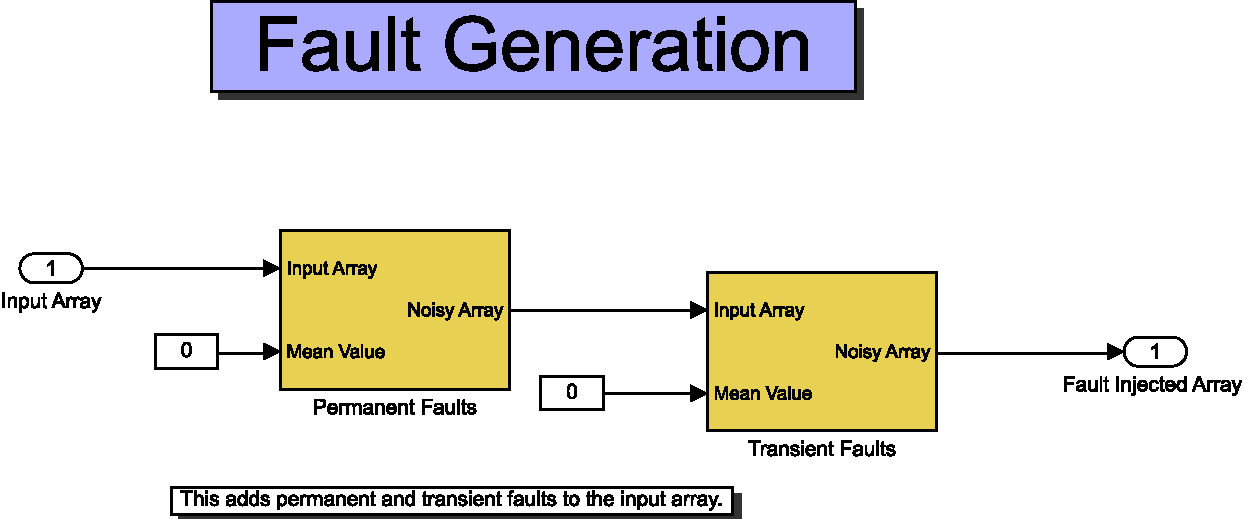
\includegraphics[width=\linewidth]{impl_dsgn_Fault Injection}}
    \\
     \subfloat[Permanent Fault Generator Block\label{fig:permanentFaultInjector}]{%
        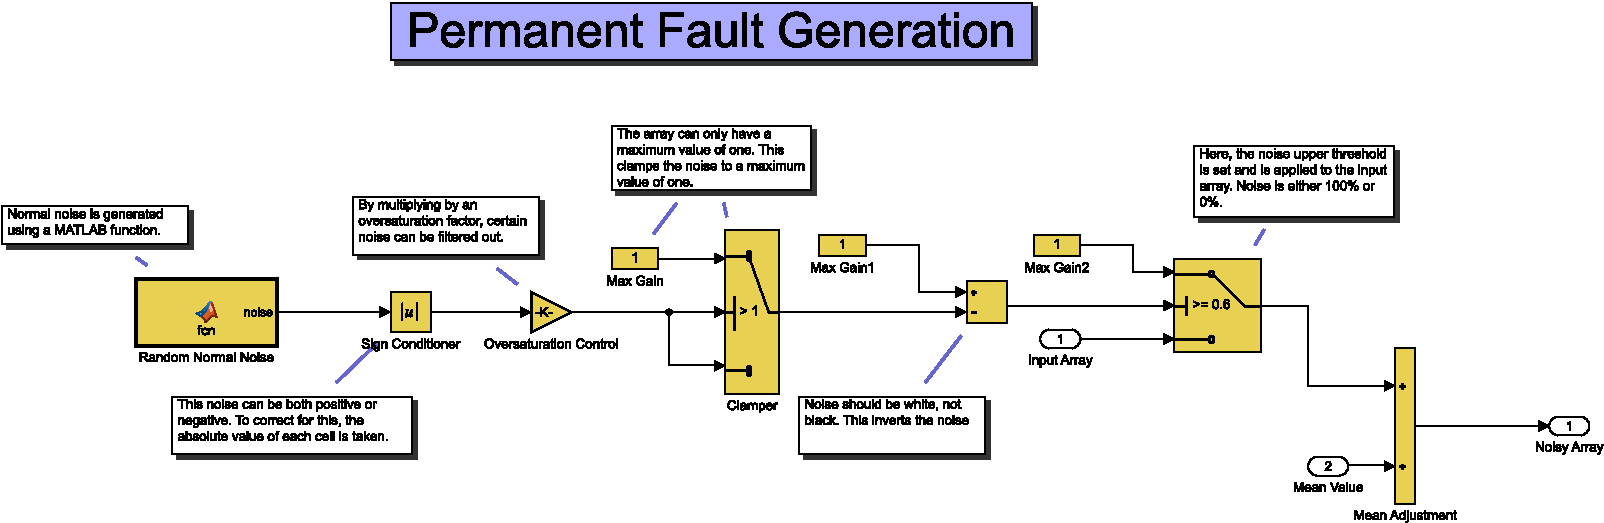
\includegraphics[width=\linewidth]{impl_dsgn_Fault Injection_Permanent Faults}}
    \caption{(a), (b) Shown are the top level fault injection block and the permanent fault injection block. The transient fault injection block is visually identical to the permanent fault injection block. The difference is inside of the MATLAB\textregisteredmark\ function block, and therefore was omitted.}
    \label{fig:faultInjection}
\end{figure}
\par As shown in Fig. \ref{fig:topLevelFaultInjector}, the reference video frame is fed into the permanent fault injection block and then is fed into the transient fault injection block. Both the transient fault and permanent fault overlays are calculated each frame which results in an decrease in real-time performance of the demo. The transient fault injection block accounted for approximately 70\% of the total execution time followed next by the permanent fault injection block at approximately 4\% of the total execution time.
\par Faults are generated using the MATLAB\textregisteredmark\ \verb!randn! function. For the permanent faults, the seed is set to a fixed value of 100, and for the transient faults, the seed is set to \verb!shuffle! which sets the seed based off the current time to provide different noise each frame. This function is hard-coded to output a 400x400 matrix due to limitations in SIMULINK\textregisteredmark. The output of this matrix are values from the standard distribution, which can output both positive and negative values. Since pixel faults can only be positive, the output matrix is corrected using an absolute value block. Next, since the maximum grey-scale value is one, a clamping block clamps the noise values to a maximum of one. The over-saturation control allows for more or less faults in the output matrix.
\par Until this point, the noise is black. The value one is subtracted from each cell in the matrix to invert the color (and make each value white). After this, the simulated image faults are added to the input array. Since a pixel can only be "on" or "off", a switch is used to selectively turn pixels on or off depending on the noise value threshold. Lastly, a mean value adjustment can be applied to the output matrix. For this application, the mean was set to zero so as not to alter the original image catastrophically.

\subsubsection{Fault Correction Sub module}
Fault Correction is accomplished by using a modified median filter.
\begin{figure}[H]
    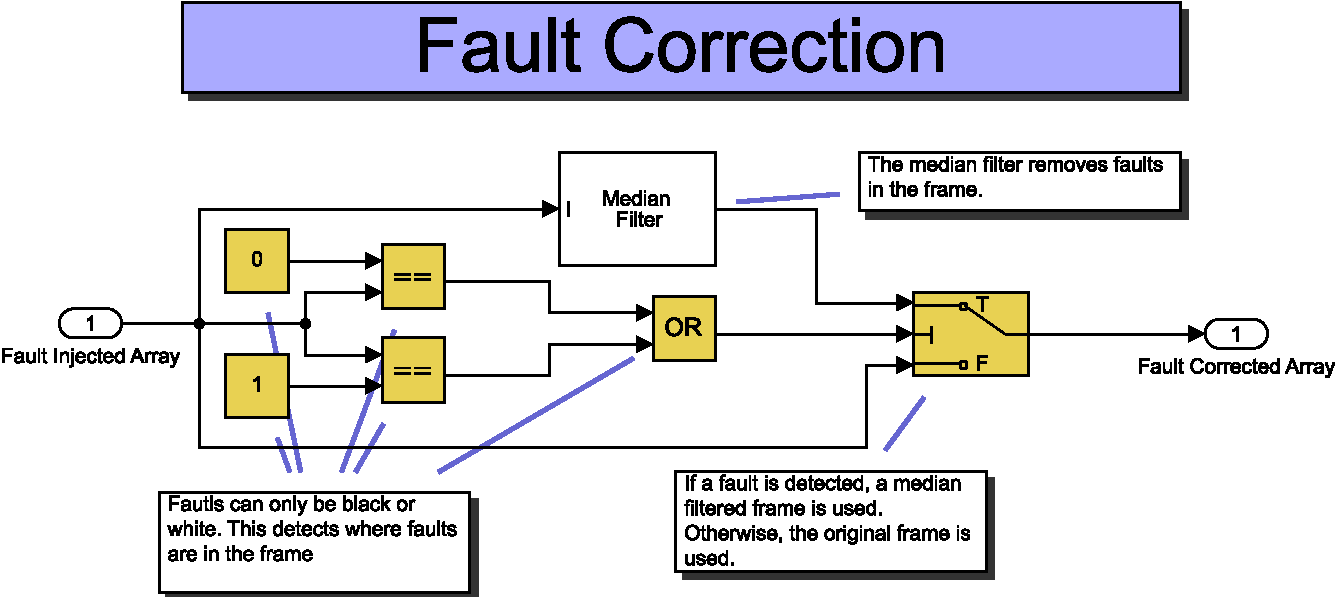
\includegraphics[width=\linewidth]{impl_dsgn_Fault Correction}
    \caption{Fault Correction using a modified median filter}
    \label{fig:medianFilter}
\end{figure}
 \par Each pixel of the input frame is checked to see if it is pure black or white to determine if a fault is present in that location. To reduce faults in the image, a median filter\footnote{For reference on median filters, please reference \hyperlink{https://homepages.inf.ed.ac.uk/rbf/HIPR2/median.htm}{Spatial Filters - Median Filters by Robert Fisher, Simon Perkins, Ashley Walker, Erik Wolfart}} is used with neighborhood size of 3x3. \autoref{fig:medianFilter} outlines the construction of this fault correction system. Since this is a somewhat idealized proof of concept design, the pixel must meet the pure white or pure black criteria. In a more real life scenario, some margin should be factored to compensate for noise in transmission to the processing unit.
 \par If the pixel is not deemed to be a fault, then the original pixel is passed through. However, if the pixel is deemed to be noisy,  then the median filtered pixel is passed through.
 \subsubsection{Fault Identification Sub module}
 Fault Identification is accomplished by averaging eight frames and isolating the parts of the frame that is the most common amongst the eight frames.
 \begin{figure}[H]
    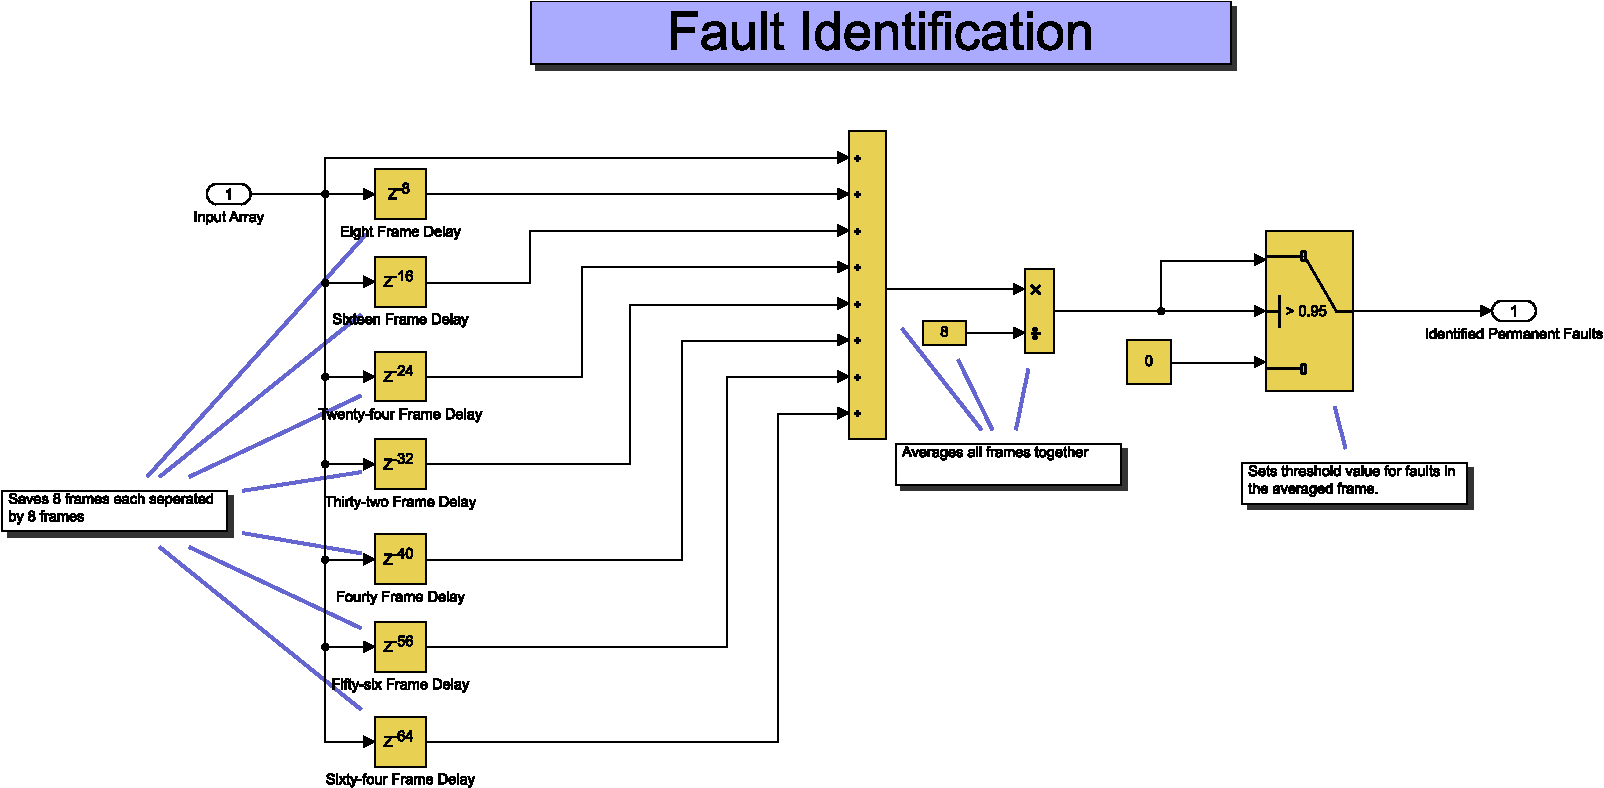
\includegraphics[width=\linewidth]{impl_dsgn_Fault Identification}
    \caption{Fault Identification}
    \label{fig:faultID}
\end{figure}
Eight frames are captured, each offset by eight frames as shown in \autoref{fig:faultID}. Because of the offset, it takes sixty-four frames to achieve accurate results. All eight frames are averaged and each pixel value is queried to determine if it meets the criteria for a permanent fault, as shown using the switch to the right of \autoref{fig:faultID}. The output of this module is the identified faults. This is fed into a video overlay block to overlay red dots for each occurrence of a permanent fault in the reference video with faults injected.

\par The permanent fault count is also captured. This is done in the permanent fault count block, as outlined in \autoref{fig:permanentFaultCount}. This block operates similarly to the fault Identification verification, except noise is identified with a switch to set the noise threshold level.
 \begin{figure}[H]
    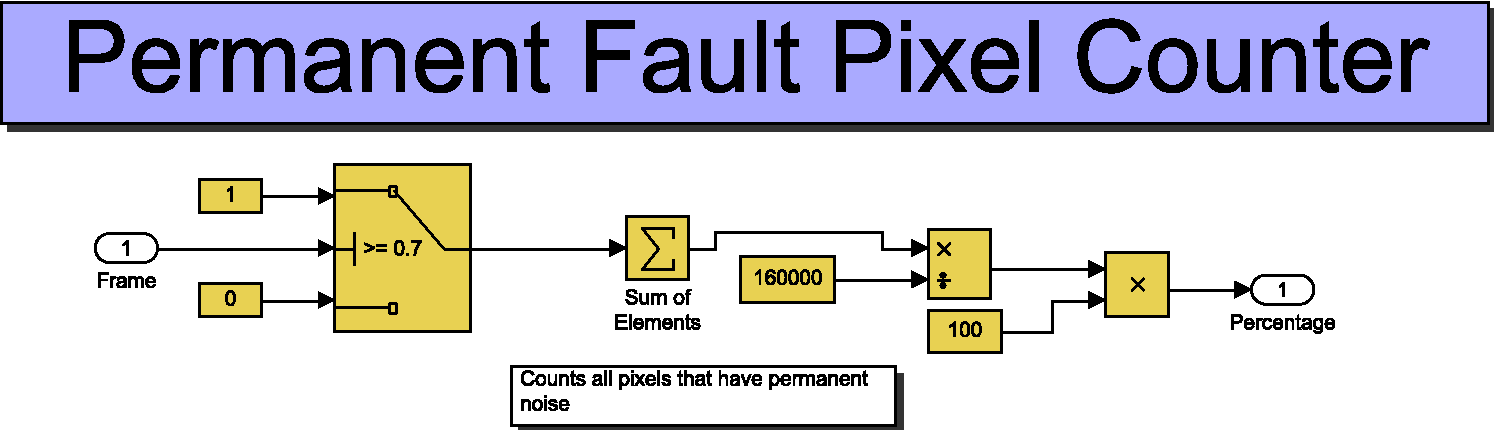
\includegraphics[width=\linewidth]{impl_dsgn_Permanent Fault Count}
    \caption{Permanent Fault Count Block}
    \label{fig:permanentFaultCount}
\end{figure}
\section{Results}
This section is split into sections describing the verification process for each module and an analysis and discussion of the overall results from the simulation.
\subsection{Verification}
\par Noise Identification Verification is done by comparing the current frame to the previous frame. The percent difference is captured and overlaid onto the output video as shown in Fig. \ref{fig:noiseIDVer}. A one unit delay block is fed as the \verb!Test! input of this block.
 \begin{figure}[H]
    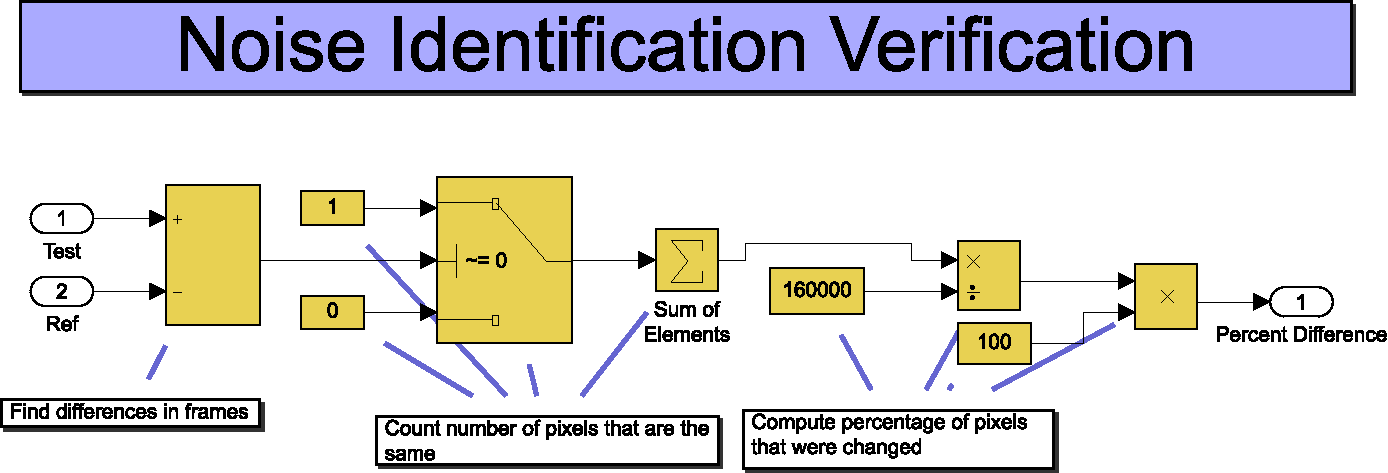
\includegraphics[width=\linewidth]{impl_dsgn_Noise Identification Verification}
    \caption{Noise Identification Verification}
    \label{fig:noiseIDVer}
\end{figure}

\par This module is verified using the peak signal-to-noise-ratio compared to the reference image. This is done in the \verb!Verification! block. The PSNR is calculated using the mean-square-error or MSE. The MSE represents the amount the reference image differs from the test image, and PSNR is a measure of the peak error and is calculated by dividing the maximum data type range by the MSE. This document uses floating point, therefore the maximum range is one\cite{mathworks}.
\section{Conclusion}
\par Further work can be done to produce HDL code or package the SIMULINK\textregisteredmark\ model into an IP package for deployment on an FPGA. Modules in \autoref{fig:sysSpecs} with a yellow background color are made with HDL blocks. Input and output blocks will have to be modified to support the correct data as well as certain SIMULINK\textregisteredmark\ computer vision blocks that performed parts of the video reading, processing, and output. However, this addition could make this model a viable option to flash onto an FPGA. This implemented design could be the truth model for any implemented IP. This method to remove noise from images has potential in harsh environments to make image sensors more reliable. For critical systems such as star trackers, however, radiation hardening the CMOS sensor would be necessary to meet customer requirements. This cost-effective solution would be suitable for applications such as standard cameras on spacecraft (such as the cameras used by astronauts aboard the International Space Station) and control cameras at nuclear plants. This would allow for more reliable imaging for the types of errors that are expected in those environments and allow for an effective longer lifetime of the sensors in these systems. Software correction is a viable alternative to radiation hardening image sensors in low cost, low risk environments.

\bibliographystyle{IEEEtran}
{\footnotesize
\bibliography{IEEEabrv,refs}
}

\end{document}